%==============================================================================
%  Congress slides (10-15 min) for:
%  A Thermodynamically-Consistent MeshGraphNet Surrogate for Transient
%  Welding Heat Transfer
%
%  Beamer, Madrid theme, blue, 16:9. Self-contained; figures expected next to
%  this .tex (already copied into docs/paper/):
%     spiral_pf_best_ep60_thermal_history.png
%     ablation_figure.png
%     compare_val_sim001_fem_on_off.png
%==============================================================================
\documentclass[aspectratio=169,11pt]{beamer}

\usetheme{Madrid}
\usecolortheme{default}        % Madrid default structure colour is blue
\setbeamertemplate{navigation symbols}{}
\setbeamertemplate{caption}[numbered]

\usepackage[utf8]{inputenc}
\usepackage[T1]{fontenc}
\usepackage{lmodern}
\usepackage{amsmath,amssymb,bm,mathtools}
\usepackage{booktabs}
\usepackage{multirow}
\usepackage{siunitx}
\usepackage{graphicx}
\usepackage{animate}
\usepackage{tikz}
\usetikzlibrary{arrows.meta,positioning,fit,backgrounds,calc,overlay-beamer-styles}

\graphicspath{{./}{./figs/}}

% --- block-diagram styles -----------------------------------------------------
\definecolor{nnblue}{rgb}{0.20,0.40,0.70}      % learned (neural) blocks
\definecolor{physgray}{rgb}{0.93,0.93,0.90}    % parameter-free physics
\tikzset{
  nn/.style={rounded corners=2pt, draw=nnblue!80, fill=nnblue!18, line width=0.7pt,
             align=center, inner sep=4pt, font=\small},
  phys/.style={rounded corners=2pt, draw=black!45, fill=physgray, line width=0.6pt,
               align=center, inner sep=4pt, font=\small},
  io/.style={align=center, font=\small\itshape},
  flow/.style={-{Latex[length=2mm]}, line width=0.8pt, draw=black!70},
  % pipeline stages (for the "data -> loss" roadmap slide)
  pipe/.style={rounded corners=3pt, draw=#1!70, fill=#1!12, line width=0.8pt,
               align=center, inner sep=4pt, text width=2.35cm, minimum height=2.2cm,
               font=\small},
  pipearr/.style={-{Latex[length=2.4mm]}, line width=1pt, draw=black!55},
}

% --- macros (match the paper) -------------------------------------------------
\newcommand{\dd}{\mathrm{d}}
\newcommand{\T}{\mathsf{T}}
\newcommand{\grad}{\nabla}
\newcommand{\Lw}{\bm{L}_{\!w}}
\newcommand{\bmu}{\bm{\mu}}
\newcommand{\cpapp}{c_p^{\mathrm{app}}}
\newcommand{\Tinf}{T_{\infty}}
\newcommand{\softplus}{\operatorname{softplus}}
\newcommand{\abs}[1]{\left\lvert#1\right\rvert}

% include an image only if present, else a labelled placeholder box (so the deck
% compiles before the user drops in the file).
\newcommand{\imgIfExists}[2]{%
  \IfFileExists{#1}{\includegraphics[width=#2\linewidth]{#1}}{%
    \fbox{\parbox[c][0.40\linewidth][c]{#2\linewidth}{\centering\ttfamily
      [imagen]\\ poner \detokenize{#1}}}}}

% block signpost: a small right-aligned pill at the top of the body (white
% background) tinted in the pipeline block colour, so it reads well and links
% each section to its block. Usage: \blocktag{basecolour}{N}{Name}
\newcommand{\blocktag}[3]{\par\vspace{-3.5mm}\hfill
  {\footnotesize\setlength{\fboxsep}{2.2pt}%
   \colorbox{#1!16}{\textcolor{#1!60!black}{\textbf{Block~#2~\textbullet~#3}}}}%
  \par\vspace{0.3mm}}
\newcommand{\restag}[1]{\par\vspace{-3.5mm}\hfill
  {\footnotesize\setlength{\fboxsep}{2.2pt}%
   \colorbox{black!8}{\textcolor{black!55}{\textbf{Results~\textbullet~#1}}}}%
  \par\vspace{0.3mm}}

% slightly tighter blocks
\setbeamersize{text margin left=1.2em,text margin right=1.2em}

\title[Structure-Preserving DL for Welding]{%
  Towards Structure-Preserving Deep Learning for Welding:\\
  A GENERIC-based Graph Network Approach}
\author[D.\ Canales et al.]{%
  D.\ Canales,\ \ B.\ Ronquillo,\ \ A.\ Dur\'an-Rosal,\ \ D.\ Gonz\'alez,\ \ E.\ Cueto}
\institute[]{Universidad Loyola \quad\textbullet\quad Universidad de Zaragoza}
\date[CMN 2026]{CMN 2026, Gij\'on \quad\textbullet\quad 1 July 2026}
% vertically aligned by content centroid (Loyola 0.52, UZ 0.39 from top)
\titlegraphic{%
  \raisebox{-0.48\height}{
\includegraphics[height=1.15cm]{logo_loyola_crop.png}}%
  \hspace{1.8cm}%
  \raisebox{-0.61\height}{
\includegraphics[height=1.15cm]{logo_uz.png}}}

\begin{document}

%------------------------------------------------------------------ 1. title
\begin{frame}[plain]
  \titlepage
\end{frame}

%------------------------------------------------------------------ 2a. computational welding
\begin{frame}{Computational welding simulation}
  \begin{columns}[c]
    \begin{column}{0.55\textwidth}
      Finite-element \textbf{weld simulation} is an established tool in
      manufacturing design, widely used across commercial \& research codes.
      \medskip\pause
      \begin{itemize}\itemsep4pt
        \item \textbf{Multiphysics:} thermal $\to$ mechanical (residual stresses,
          distortion) $\to$ metallurgy (microstructure, phase fractions).
        \item High fidelity, but a single nonlinear transient run costs
          \textbf{minutes to hours}.
        \item<3-> Large \textbf{design-space exploration}, optimization,
          uncertainty quantification and online control become \textbf{prohibitive}.
      \end{itemize}
    \end{column}
    \begin{column}{0.45\textwidth}
      \centering
      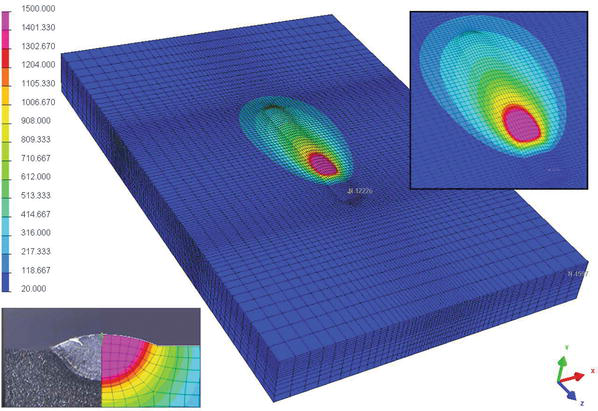
\includegraphics[width=\linewidth]{welding_image.png}\\[2pt]
      {\scriptsize 3D thermal weld FEM: moving melt pool.}
    \end{column}
  \end{columns}
\end{frame}

%------------------------------------------------------------------ 2b. learned surrogate + challenges
\begin{frame}{Learned surrogates: MeshGraphNet \& its challenges}
  \begin{columns}[T]
    \begin{column}{0.56\textwidth}
      Mesh-based learned surrogates, e.g.\ \textbf{MeshGraphNet} (MGN), are
      promising: fast, operate on the simulation mesh, roll forward
      autoregressively.
      \medskip\pause

      \textbf{Without physics, two limitations:}
      \begin{enumerate}\itemsep3pt
        \item<3-> error \textbf{accumulates} over long rollouts: unstable,
          generalizes worse;
        \item<4-> need \textbf{more training data}, so training is costly.
      \end{enumerate}
      \onslide<5->{\medskip
      \structure{\small We embed physics (structure-preserving) for stable,
      data-efficient generalization.}}
    \end{column}
    \begin{column}{0.44\textwidth}
      \centering
      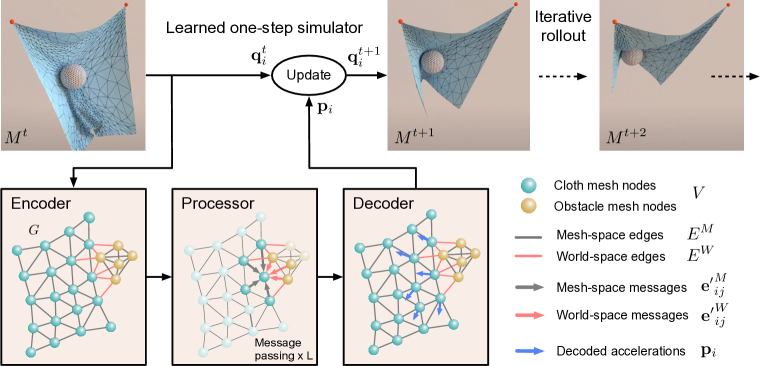
\includegraphics[width=\linewidth]{mgn.png}\\[3pt]
      {\scriptsize MeshGraphNet, Pfaff et al., DeepMind (2021)}
    \end{column}
  \end{columns}
\end{frame}

%------------------------------------------------------------------ pipeline roadmap (after intro)
\begin{frame}{The pipeline: from FEM data to the training loss}
  \vspace{2mm}
  \centering
  \resizebox{\textwidth}{!}{%
  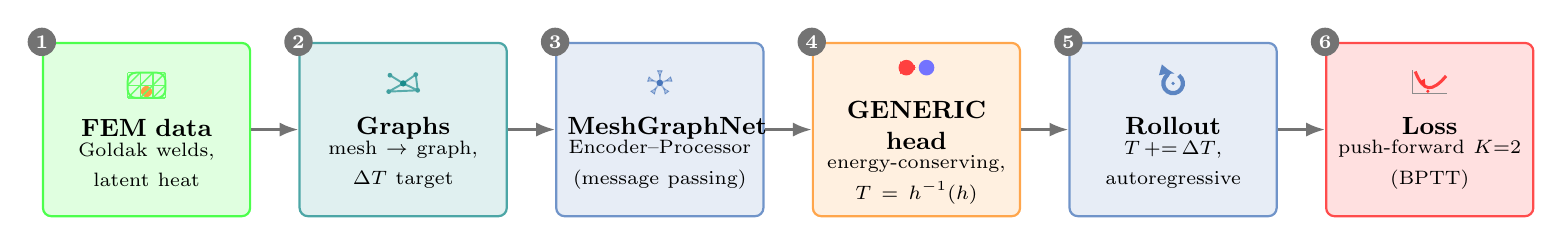
\begin{tikzpicture}[node distance=6mm,
    numbadge/.style={circle, fill=black!55, text=white, font=\bfseries\scriptsize,
                     inner sep=1.1pt, minimum size=3.6mm}]
    % --- stages (revealed one by one) ---
    \node[pipe=green] (s1) {%
      \tikz[scale=0.16]{\useasboundingbox (0,0) rectangle (3,2);
        \fill[green!12] (0,0) rectangle (3,2);
        \fill[orange!75] (1,0) rectangle (2,1);          % hot weld zone
        \foreach \x in {0,1,2,3} \draw[green!60,line width=0.5pt] (\x,0)--(\x,2);
        \foreach \y in {0,1,2} \draw[green!60,line width=0.5pt] (0,\y)--(3,\y);
        \foreach \x in {0,1,2} \foreach \y in {0,1}
          \draw[green!60,line width=0.5pt] (\x,\y)--(\x+1,\y+1);
        \draw[green!65,line width=0.7pt] (0,0) rectangle (3,2);}\\[3pt]
      \textbf{FEM data}\\[-1pt]{\scriptsize Goldak welds,\\ latent heat}};
    \node[pipe=teal, right=of s1, visible on=<2->] (s2) {%
      \tikz[scale=0.16]{\useasboundingbox (0,0) rectangle (3,2);
        \coordinate (na) at (0.35,0.35); \coordinate (nb) at (2.65,0.45);
        \coordinate (nc) at (1.5,1.0); \coordinate (nd) at (2.5,1.7);
        \coordinate (ne) at (0.45,1.65);
        \draw[teal!65,line width=0.7pt] (na)--(nc) (nc)--(nb) (nc)--(nd)
          (nc)--(ne) (nb)--(nd) (na)--(nb);
        \foreach \n in {na,nb,nd,ne} \fill[teal!75] (\n) circle(0.19);
        \fill[teal!90] (nc) circle(0.25);}\\[3pt]
      \textbf{Graphs}\\[-1pt]{\scriptsize mesh $\to$ graph,\\ $\Delta T$ target}};
    \node[pipe=nnblue, right=of s2, visible on=<3->] (s3) {%
      \tikz[scale=0.16]{\useasboundingbox (0,0) rectangle (3,2);
        \begin{scope}[shift={(1.5,1)}]
        \foreach \a in {18,90,162,234,306}{
          \draw[nnblue!45,line width=0.6pt] (0,0)--(\a:0.82);
          \draw[-{Latex[length=1mm]},nnblue!75,line width=0.7pt] (\a:0.78) -- (\a:0.36);
          \fill[nnblue!45] (\a:0.82) circle(0.14);}
        \fill[nnblue!90] (0,0) circle(0.26);\end{scope}}\\[3pt]
      \textbf{MeshGraphNet}\\[-1pt]{\scriptsize Encoder--Processor\\ (message passing)}};
    \node[pipe=orange, right=of s3, visible on=<4->] (s4) {%
      \tikz[scale=0.16]{\useasboundingbox (0,0) rectangle (3,2);
        \fill[red!75] (0.7,1) circle(0.62);                        % hot
        \fill[blue!55] (2.3,1) circle(0.62);                       % cold
        \draw[-{Latex[length=2.2mm]},red!75,line width=1.6pt] (1.42,1) -- (1.58,1);}\\[3pt]
      \textbf{GENERIC head}\\[-1pt]{\scriptsize energy-conserving,\\ $T=h^{-1}(h)$}};
    \node[pipe=nnblue, right=of s4, visible on=<5->] (s5) {%
      \tikz[scale=0.16]{\useasboundingbox (0,0) rectangle (3,2);
        \begin{scope}[shift={(1.5,1)}]
        \draw[-{Latex[length=2mm]},nnblue!80,line width=1.5pt] (55:0.78) arc (55:-285:0.78);
        \fill[nnblue!80] (0,0) circle(0.14);\end{scope}}\\[3pt]
      \textbf{Rollout}\\[-1pt]{\scriptsize $T\,{+}{=}\,\Delta T$,\\ autoregressive}};
    \node[pipe=red, right=of s5, visible on=<6->] (s6) {%
      \tikz[scale=0.16]{\useasboundingbox (0,0) rectangle (3,2);
        \draw[black!45,line width=0.5pt] (0.15,0.15)--(2.9,0.15);   % axes
        \draw[black!45,line width=0.5pt] (0.15,0.15)--(0.15,2.0);
        \draw[red!75,line width=1.1pt]
          (0.35,1.9) .. controls (1.0,0.25) and (1.7,0.25) .. (2.8,1.55);
        \fill[red!80] (1.35,0.33) circle(0.14);                     % minimum
        \draw[-{Latex[length=1.2mm]},red!80,line width=0.7pt] (0.9,1.15)--(1.25,0.55);}\\[3pt]
      \textbf{Loss}\\[-1pt]{\scriptsize push-forward $K{=}2$\\ (BPTT)}};

    % --- arrows ---
    \draw[pipearr, visible on=<2->] (s1) -- (s2);
    \draw[pipearr, visible on=<3->] (s2) -- (s3);
    \draw[pipearr, visible on=<4->] (s3) -- (s4);
    \draw[pipearr, visible on=<5->] (s4) -- (s5);
    \draw[pipearr, visible on=<6->] (s5) -- (s6);
    % --- numbered badges (tie to the "Block N" section tags) ---
    \node[numbadge, visible on=<1->] at (s1.north west) {1};
    \node[numbadge, visible on=<2->] at (s2.north west) {2};
    \node[numbadge, visible on=<3->] at (s3.north west) {3};
    \node[numbadge, visible on=<4->] at (s4.north west) {4};
    \node[numbadge, visible on=<5->] at (s5.north west) {5};
    \node[numbadge, visible on=<6->] at (s6.north west) {6};
  \end{tikzpicture}}

  \vfill
  {\centering\small\structure{\textbf{Our proposal:} a MeshGraphNet thermal
  surrogate with a structure-preserving \emph{enthalpy-GENERIC} head
  (energy-conserving, entropy-producing), trained with \emph{push-forward} for
  stable long autoregressive rollouts.}\par}
\end{frame}

%------------------------------------------------------------------ Block 1: FEM data — physics
\begin{frame}{Governing physics and the FEM ground truth}
  \blocktag{green!55!black}{1}{FEM data \& dataset}
  Transient heat conduction with a moving Goldak arc source:
  \begin{equation*}
    \rho\,\cpapp(T)\,\frac{\partial T}{\partial t}
      = \grad\!\cdot\!\big(k(T)\,\grad T\big) + Q(\bm x,t).
  \end{equation*}
  $\cpapp(T)$: \textbf{apparent heat capacity} (folds in latent heat; enthalpy
  $h(T)=\rho\!\int\cpapp\,\dd\tau$). \ Robin / Dirichlet boundaries.
  \pause

  \textbf{FEM} ($P_1$ triangles) $\to$ semidiscrete system, advanced by the
  $\theta$-method (backward Euler):
  \begin{equation*}
    \bm M(T)\,\dot{\bm T}+\bm A(T)\,\bm T=\bm b(t)
    \quad\Longrightarrow\quad
    \Big(\tfrac{1}{\Delta t}\bm M+\bm A\Big)\bm T^{\,n+1}
      =\tfrac{1}{\Delta t}\bm M\,\bm T^{\,n}+\bm b^{\,n+1}.
  \end{equation*}
  \pause
  {\small $\bm M$ (mass, $\rho\cpapp$),\ \ $\bm A=\bm K+\bm R$ (conduction $+$
  Robin),\ \ $\bm b$ (Goldak $+$ boundary loads);\ \ Picard for the
  nonlinearity.}
\end{frame}

%------------------------------------------------------------------ 3b. training dataset
\begin{frame}{The training dataset}
  \blocktag{green!55!black}{1}{FEM data \& dataset}
  \begin{center}
    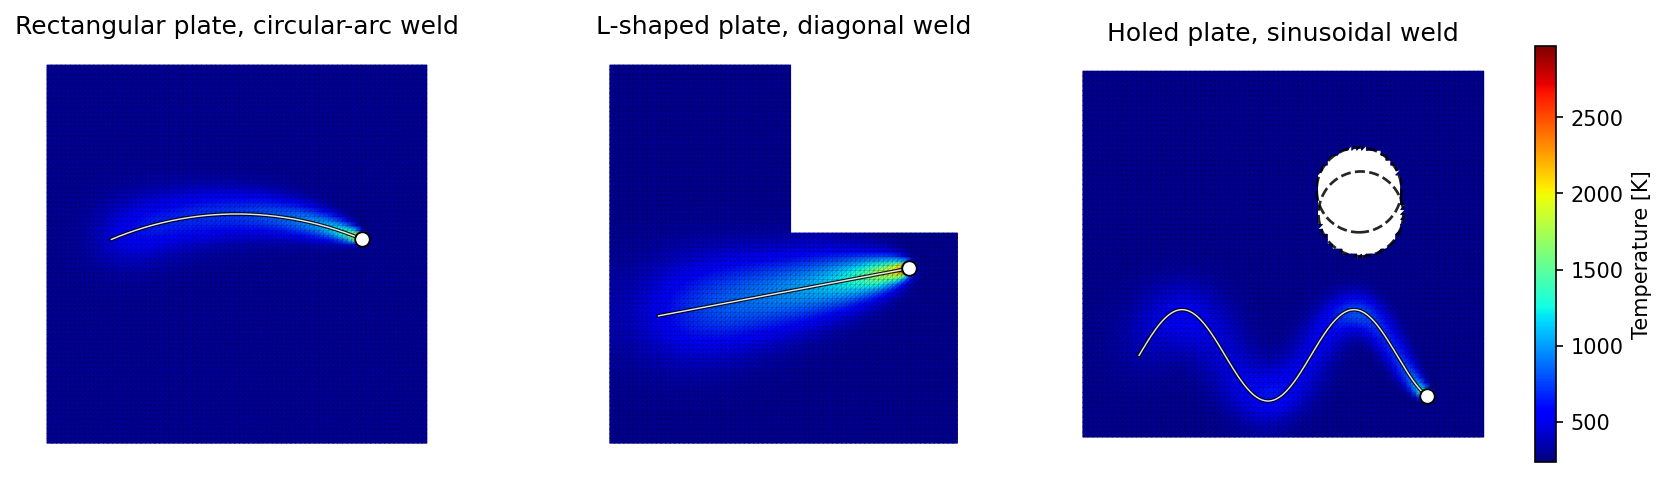
\includegraphics[width=0.80\linewidth]{dataset_samples.png}
  \end{center}
  \vspace{-1.5mm}
  {\footnotesize \textbf{\num{360} FEM simulations} (\num{300} train / \num{60}
  val, split by simulation), \num{398597} snapshot pairs;\ \ $P_1$ mesh at
  \SI{3}{mm} ($\sim$\numrange{0.8}{6.6}k nodes).}
  \pause
  \vspace{0.5mm}

  {\footnotesize\centering\renewcommand{\arraystretch}{1.1}
  \begin{tabular}{@{}ll@{\hspace{2.2em}}ll@{}}
    \textbf{Geometry} & rect.\ / L-shape / holed &
      \textbf{Trajectory} & straight, diagonal, sinusoid, arc \\
    \textbf{Plate size} & \SIrange{80}{250}{mm} &
      \textbf{Power} & \SIrange{1.5}{3.5}{kW},\ $\eta\in[0.70,0.90]$ \\
    \textbf{Travel speed} & \SIrange{2}{12}{mm/s} &
      \textbf{Thickness} & \SIrange{4}{8}{mm} \\
    \textbf{Ambient} & \SIrange{290}{320}{K} &
      \textbf{Boundary} & $h_{\mathrm{conv}}\,\SIrange{5}{40}{W/m^2K}$,\ $\varepsilon\in\{0,0.2,0.35\}$ \\
  \end{tabular}}
\end{frame}

%------------------------------------------------------------------ Block 2: graph representation
\begin{frame}{From FEM snapshots to graphs}
  \blocktag{teal!70!black}{2}{Graph representation}
  \textbf{One graph per snapshot pair} $T^t\!\to\!T^{t+1}$: mesh nodes $=$ graph
  nodes, mesh edges (both directions) $=$ graph edges.
  \medskip

  \begin{columns}[T]
    \begin{column}{0.46\textwidth}
      \centering
      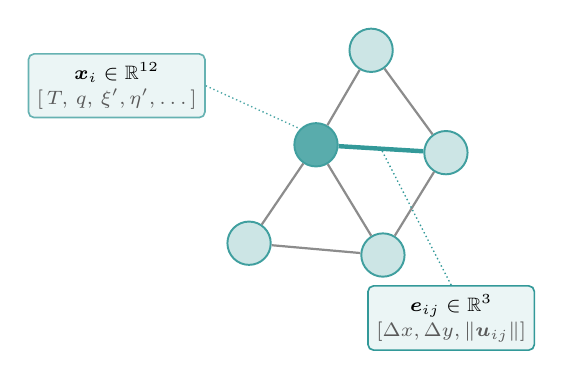
\begin{tikzpicture}[
        gnode/.style={circle, draw=teal!75, fill=teal!20, line width=0.7pt,
                      minimum size=5.5mm, inner sep=0pt},
        gedge/.style={draw=black!45, line width=0.8pt},
        chip/.style={rounded corners=2pt, draw=teal!60, fill=teal!8,
                     line width=0.6pt, font=\scriptsize, align=center, inner sep=3pt},
        lead/.style={draw=teal!70, line width=0.5pt, densely dotted}]
        % mesh patch
        \node[gnode] (a) at (0,0) {};
        \node[gnode] (b) at (1.7,-0.15) {};
        \node[gnode, fill=teal!65] (c) at (0.85,1.25) {};
        \node[gnode] (d) at (2.5,1.15) {};
        \node[gnode] (f) at (1.55,2.45) {};
        \draw[gedge] (a)--(b); \draw[gedge] (a)--(c); \draw[gedge] (b)--(d);
        \draw[gedge] (c)--(f); \draw[gedge] (d)--(f);
        \draw[gedge] (b)--(c);
        \draw[gedge, draw=teal!80, line width=1.6pt] (c)--(d);  % highlighted edge
        % node feature chip
        \node[chip, anchor=east] (xchip) at (-0.55,2.0)
          {$\bm x_i\in\mathbb{R}^{12}$\\[1pt]\color{black!65}$[\,T,\,q,\,\xi',\eta',\dots\,]$};
        \draw[lead] (xchip.east) -- (c.north west);
        % edge feature chip
        \node[chip, anchor=west, draw=teal!80] (echip) at (1.5,-0.95)
          {$\bm e_{ij}\in\mathbb{R}^{3}$\\[1pt]\color{black!65}$[\Delta x,\Delta y,\lVert\bm u_{ij}\rVert]$};
        \draw[lead, draw=teal!80] (echip.north) -- ($(c)!0.5!(d)$);
      \end{tikzpicture}
    \end{column}
    \begin{column}{0.54\textwidth}
      \small
      \begin{itemize}\itemsep4pt
        \item<2-> \textbf{Node} $\bm x_i$ (12-d): $T$, Goldak source $q$, co-moving
          torch coords, process \& boundary scalars.
        \item<3-> \textbf{Edge} $\bm e_{ij}$ (3-d): \emph{relative} displacement
          only; no absolute coordinates, generalizes across meshes.
        \item<4-> \textbf{Target} $\bm y=\Delta T=T^{t+1}-T^{t}$ (per node).
      \end{itemize}
    \end{column}
  \end{columns}
\end{frame}

%------------------------------------------------------------------ Block 3: encoder-processor
\begin{frame}{The MeshGraphNet: Encoder--Processor}
  \blocktag{nnblue}{3}{MeshGraphNet (MPNN)}
  \textbf{Encoder.} Two MLPs lift raw node/edge features to a shared latent of
  width $d{=}128$:
  \begin{equation*}
    \bm v_i^{(0)}=\mathrm{MLP}_{\mathrm{enc}}^{v}(\bm x_i),\qquad
    \bm\epsilon_{ij}^{(0)}=\mathrm{MLP}_{\mathrm{enc}}^{e}(\bm e_{ij}).
  \end{equation*}
  \pause
  \textbf{Processor.} $L{=}8$ message-passing blocks with \emph{residual} updates:
  \begin{align*}
    \bm\epsilon_{ij}&\leftarrow \bm\epsilon_{ij}
       +\mathrm{MLP}_e\big([\,\bm\epsilon_{ij},\bm v_i,\bm v_j\,]\big), &&\text{(edge update)}\\[-1pt]
    \bm m_j&=\textstyle\sum_{i\in\mathcal N(j)}\bm\epsilon_{ij}, &&\text{(sum aggregation)}\\[-1pt]
    \bm v_j&\leftarrow \bm v_j+\mathrm{MLP}_v\big([\,\bm v_j,\bm m_j\,]\big). &&\text{(node update)}
  \end{align*}
  \pause
  After $L{=}8$ hops each node ``sees'' up to 8 edges away (the heat-affected zone);
  $\approx$\,\num{1.29}\,M params. \quad\structure{\small A standard decoder would map
  $\bm v_i\!\to\!\Delta T$; we \emph{replace} it with the GENERIC head (next).}
\end{frame}

%------------------------------------------------------------------ 5. GENERIC framework -> dissipative
\begin{frame}{GENERIC: from the general form to pure dissipation}
  \blocktag{orange!80!black}{4}{Enthalpy-GENERIC head}
  \textbf{Classic GENERIC.} Any dynamics splits into a \emph{reversible} and a
  \emph{dissipative} part, driven by energy $E$ and entropy $S$:
  \begin{equation*}
    \dot{\bm z}=\underbrace{\bm L\,\partial_{\bm z}E}_{\text{reversible}}
               +\underbrace{\bm M\,\partial_{\bm z}S}_{\text{dissipative}},
    \qquad \bm L^\T=-\bm L,\quad \bm M\ \text{SPSD},\quad
    \bm L\,\partial_{\bm z}S=\bm M\,\partial_{\bm z}E=\bm 0 .
  \end{equation*}
  \pause

  \textbf{Our case: heat conduction is purely dissipative.} There is no
  reversible heat flow, so $\bm L=\bm 0$ and only the dissipative part survives:
  \begin{equation*}
    \boxed{\;\dot{\bm z}=\bm M\,\partial_{\bm z}S\;}
  \end{equation*}
  \pause
  \centering
  \structure{Two choices left: \textbf{the state $\bm z$} and \textbf{the operator
  $\bm M$}. \\ The conserved quantity is energy, so take the state to be
  the per-node energy $\mathcal E_i=h_iV_i$ (volumetric \emph{enthalpy} $\times$
  volume), not temperature.}
\end{frame}

%------------------------------------------------------------------ 6. enthalpy-state head
% ---- 4b: the operator (chain rule -> the two laws) --------------------------
\begin{frame}{The operator $\bm M$: chain rule $\Rightarrow$ the two laws}
  \blocktag{orange!80!black}{4}{Enthalpy-GENERIC head}
  \textbf{The state is a \emph{vector}; the energy is a \emph{scalar}.}
  State $\bm z=(\mathcal E_1,\dots,\mathcal E_N)$ with
  $\mathcal E_i=h_iV_i$ (volumetric enthalpy $\times$ volume); the total-energy
  potential is $E=\sum_i\mathcal E_i=\bm 1^\T\bm z$.
  \medskip\pause

  \textbf{Chain rule} along $\dot{\bm z}=\bm M\bmu$ \ (force
  $\bmu\equiv\partial_{\bm z}S$, i.e.\ $\mu_i=\partial S/\partial\mathcal E_i=1/T_i$):
  \begin{equation*}
    \dot E=(\partial_{\bm z}E)^\T\dot{\bm z}=\bm 1^\T\bm M\bmu,
    \qquad
    \dot S=(\partial_{\bm z}S)^\T\dot{\bm z}=\bmu^\T\bm M\bmu,
    \qquad \text{since }\ \partial_{\bm z}E=\bm 1\ \ (E=\bm 1^\T\bm z).
  \end{equation*}
  \pause

  \textbf{Choose $\bm M=\Lw$}, the graph Laplacian of \emph{learned} conductances
  $w_{ij}=w_{ji}\ge0$ \ ($\Lw=\bm D-\bm W$):
  \begin{itemize}\itemsep1pt
    \item $\bm 1^\T\Lw=\bm 0$ (zero column sums) $\Rightarrow \dot E=0$
      \ \textbf{(1st law)}.
    \item $\Lw$ SPSD $\Rightarrow \dot S=\bmu^\T\Lw\bmu
      =\tfrac12\sum w_{ij}(\mu_i{-}\mu_j)^2\ge0$ \ \textbf{(2nd law)};\ heat
      hot$\to$cold.
  \end{itemize}
\end{frame}

% ---- 4c: what the head computes (the algorithm -> dT) ------------------------
\begin{frame}{What the head computes each step: the increment $\Delta T$}
  \blocktag{orange!80!black}{4}{Enthalpy-GENERIC head}
  The network must output a per-node $\Delta T$. The head builds it \emph{through
  energy} (the enthalpy method), in three steps:
  \medskip\pause

  \begin{enumerate}\itemsep3pt
    \item \textbf{Exchange energy} with neighbours (the dissipative operator),
      plus the external arc/boundary term:
      \[ \Delta\mathcal E_i=\underbrace{(\Lw\bmu)_i}_{\text{conduction}}
         +\ \Delta\mathcal E_i^{\mathrm{ext}}. \]
    \item<3-> \textbf{Update the stored energy:}\quad
      $\mathcal E_i \leftarrow \mathcal E_i+\Delta\mathcal E_i$.
    \item<4-> \textbf{Read off temperature} through the enthalpy curve:\quad
      $T_i^{\text{new}}=h^{-1}(\mathcal E_i/V_i)$,\quad
      $\boxed{\,\Delta T_i=T_i^{\text{new}}-T_i\,}$.
  \end{enumerate}
  \medskip
  \onslide<5->{\structure{\small Latent heat is \emph{exact}: at the melt pool
  $h^{-1}$ is flat, so a large $\Delta\mathcal E$ gives almost no $\Delta T$,
  just like the FEM.}}
\end{frame}

%------------------------------------------------------------------ Block 5: autoregressive rollout
\begin{frame}{Inference: autoregressive rollout}
  \blocktag{nnblue}{5}{Autoregressive rollout}
  Given only the initial field $T^0$ and the (known) torch schedule, the model
  predicts the \textbf{whole} history step by step:
  \medskip\pause

  \begin{center}
  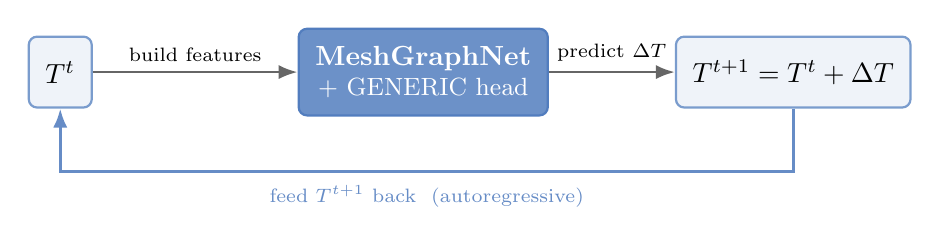
\begin{tikzpicture}[
    state/.style={rounded corners=3pt, draw=nnblue!65, fill=nnblue!8,
                  line width=0.8pt, align=center, inner sep=6pt, minimum height=9mm},
    model/.style={rounded corners=3pt, draw=nnblue!85, fill=nnblue!72,
                  text=white, line width=0.8pt, align=center, inner sep=6pt,
                  minimum height=11mm, font=\bfseries},
    fwd/.style={-{Latex[length=2.4mm]}, line width=1pt, draw=black!60},
    fb/.style={-{Latex[length=2.4mm]}, line width=1pt, draw=nnblue!75},
    node distance=16mm]
    \node[state] (t0) {$T^{t}$};
    \node[model, right=26mm of t0] (mod) {MeshGraphNet\\[-1pt]\normalfont\small $+$ GENERIC head};
    \node[state, right=of mod] (t1) {$T^{t+1}=T^{t}+\Delta T$};
    \draw[fwd] (t0) -- node[above,font=\scriptsize]{build features} (mod);
    \draw[fwd] (mod) -- node[above,font=\scriptsize]{predict $\Delta T$} (t1);
    % orthogonal feedback loop (straight segments, label on the bottom run)
    \coordinate (b1) at ($(t1.south)+(0,-8mm)$);
    \coordinate (b0) at ($(t0.south)+(0,-8mm)$);
    \draw[fb] (t1.south) -- (b1) -- (b0) -- (t0.south);
    \node[font=\scriptsize, text=nnblue!75, below=0.5mm] at ($(b1)!0.5!(b0)$)
      {feed $T^{t+1}$ back \ (autoregressive)};
  \end{tikzpicture}
  \end{center}
  \pause
  {\small
  \begin{itemize}\itemsep2pt
    \item \textbf{Only $T$ is fed back:} the schedule ($q$, co-moving coords,
      speed) is known for every step.
    \item Errors can \textbf{accumulate} over long horizons (many steps).
  \end{itemize}}
  \onslide<4->{\centering
    \structure{\small So we train on the long rollout: the push-forward
    loss (next).}}
\end{frame}

%------------------------------------------------------------------ Block 6: push-forward loss
\begin{frame}{Push-forward training: unroll $K$ steps}
  \blocktag{red!75!black}{6}{Push-forward loss}
  Minimizing the \emph{single-step} error does not guarantee a good long rollout.
  \textbf{Push-forward}: unroll the model $K$ steps, feed each prediction back, and
  train on the error over the whole window; the gradient flows through \emph{all}
  $K$ steps.
  \medskip\pause

  \begin{center}
  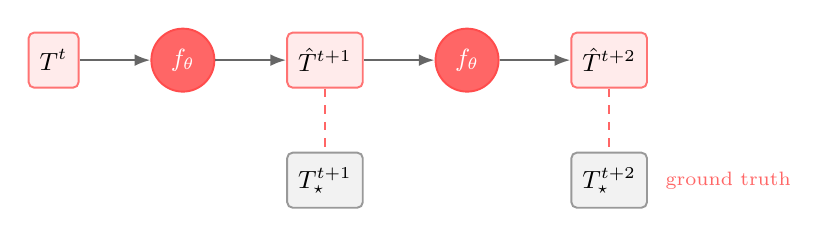
\begin{tikzpicture}[
    st/.style={rounded corners=2pt, draw=red!55, fill=red!8, line width=0.7pt,
               inner sep=4pt, minimum height=7mm, font=\small},
    gt/.style={rounded corners=2pt, draw=black!40, fill=black!5, line width=0.7pt,
               inner sep=4pt, minimum height=7mm, font=\small},
    mm/.style={circle, draw=red!70, fill=red!60, text=white, line width=0.7pt,
               inner sep=1pt, minimum size=8mm, font=\small\bfseries},
    ar/.style={-{Latex[length=2mm]}, line width=0.9pt, draw=black!60},
    cmp/.style={dashed, line width=0.7pt, draw=red!60},
    node distance=9mm]
    \node[st] (s0) {$T^{t}$};
    \node[mm, right=of s0] (f1) {$f_\theta$};
    \node[st, right=of f1] (s1) {$\hat T^{t+1}$};
    \node[mm, right=of s1] (f2) {$f_\theta$};
    \node[st, right=of f2] (s2) {$\hat T^{t+2}$};
    \draw[ar] (s0)--(f1); \draw[ar] (f1)--(s1);
    \draw[ar] (s1)--(f2); \draw[ar] (f2)--(s2);
    \node[gt, below=8mm of s1] (g1) {$T^{t+1}_\star$};
    \node[gt, below=8mm of s2] (g2) {$T^{t+2}_\star$};
    \draw[cmp] (s1)--(g1); \draw[cmp] (s2)--(g2);
    \node[font=\scriptsize, text=red!60, right=1mm of g2] {ground truth};
    \node[font=\scriptsize, right=0.5mm of f2] {};
  \end{tikzpicture}
  \end{center}
  \pause
  \begin{equation*}
    \mathcal L=\frac1K\sum_{k=1}^{K}\big\lVert\,\hat T^{t+k}-T^{t+k}_\star\,\big\rVert^2
    \qquad(\text{mean squared temperature error over the window}).
  \end{equation*}
  \pause
  \centering
  \structure{We use $\bm{K=2}$: it clearly outperformed $K=1$ on the rollout.}
\end{frame}

%------------------------------------------------------------------ Validation 1: ablation table
\begin{frame}{Ablation: thermodynamic structure ON vs.\ OFF}
  \restag{validation \& ablation}
  Identical models except the head: same $K{=}2$, split, budget, noise,
  hyperparameters, so the two are directly comparable.
  \medskip\pause

  \begin{table}
    \centering\small
    \begin{tabular}{l c c c c}
      \toprule
      & & \textbf{Held-out val.} & \multicolumn{2}{c}{\textbf{Spiral (OOD)}}\\
      & & {\scriptsize unseen, train-like} & \multicolumn{2}{c}{\scriptsize harder, out-of-distribution}\\
      \cmidrule(lr){3-3}\cmidrule(lr){4-5}
      Configuration & Params & RMSE (K) & RMSE (K) & min $T$ (K)\\
      \midrule
      \textbf{GENERIC ON}  & \num{1375238} & \textbf{34.5} & \textbf{33.2} & \textbf{287} ($-6$)\\
      \textbf{GENERIC OFF} & \num{1291777} & 46.9          & 58.6          & 140 ($-153$)\\
      \bottomrule
    \end{tabular}
  \end{table}
  \par\smallskip
  {\footnotesize Held-out validation $=$ \emph{unseen} welds drawn like the training
  set; the \emph{spiral} is a harder, out-of-distribution trajectory.}
  \medskip\pause
  \begin{itemize}
    \item<3-> \textbf{Maximum principle:} OFF cools to \SIrange{140}{190}{K}
      ($\sim$\SI{150}{K} unphysical); ON stays at the \SI{293}{K} floor.
    \item<4-> \textbf{Selectability:} for ON the best-val checkpoint \emph{is} the
      best spiral; for OFF it is not.
  \end{itemize}
\end{frame}

%------------------------------------------------------------------ Validation 2: held-out case 1
\begin{frame}{Held-out validation: thermal histories (case 1)}
  \restag{held-out validation (unseen, train-like)}
  \vfill\centering
  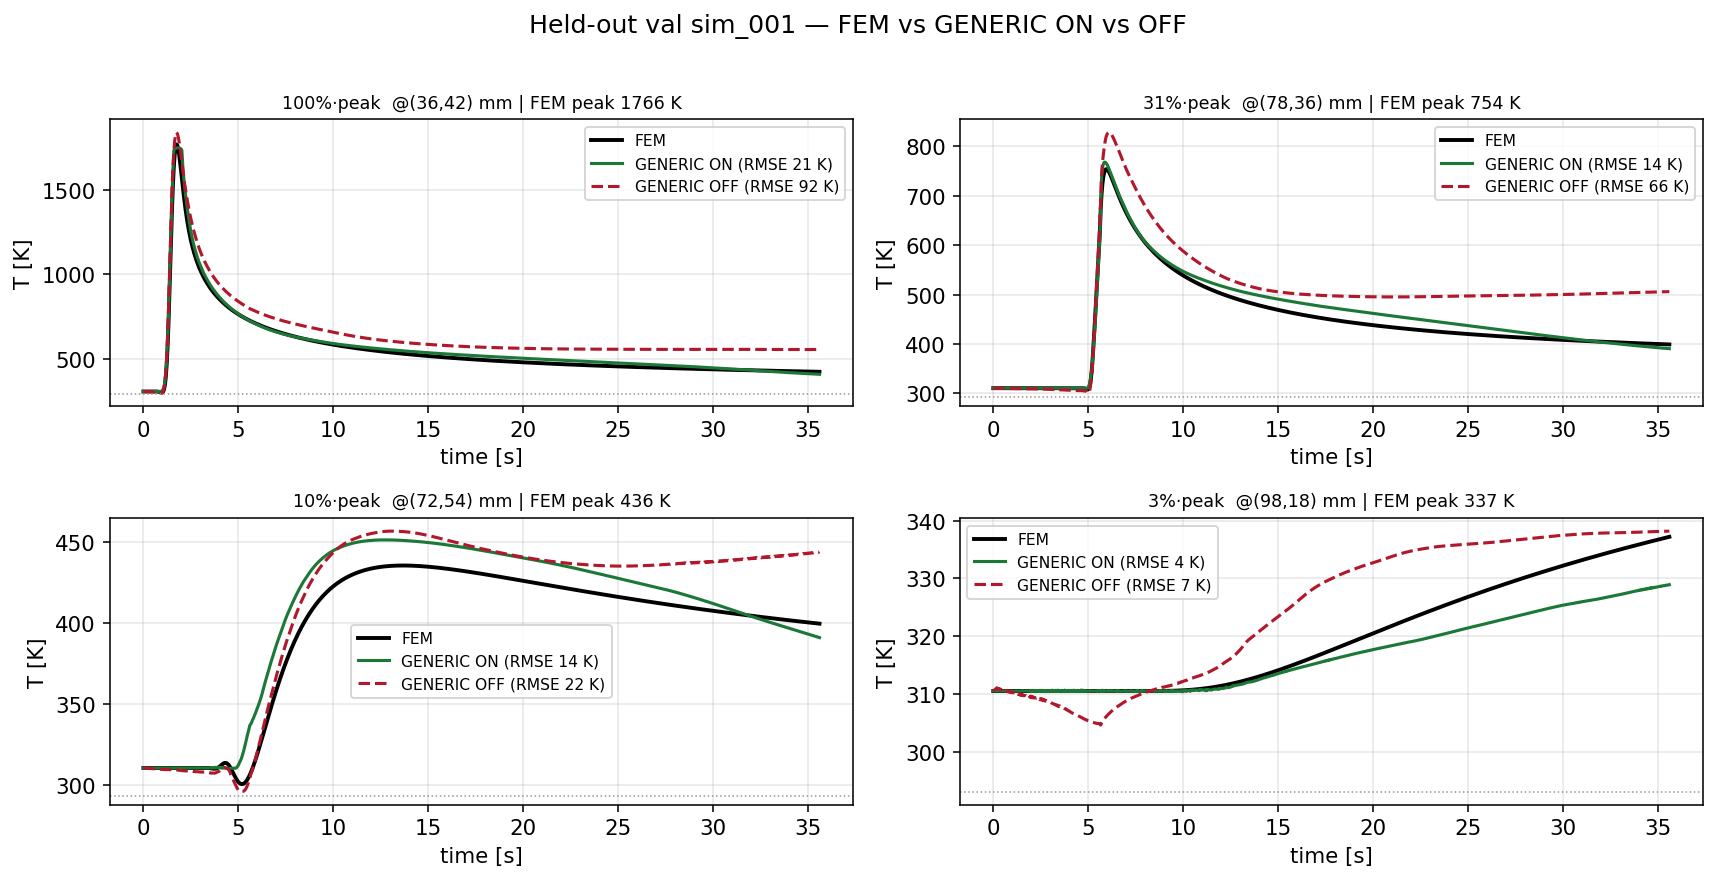
\includegraphics[width=0.92\linewidth]{compare_val_sim001_fem_on_off.png}
  \vfill
\end{frame}

%------------------------------------------------------------------ Validation 3: held-out case 2
\begin{frame}{Held-out validation: thermal histories (case 2)}
  \restag{held-out validation (unseen, train-like)}
  \vfill\centering
  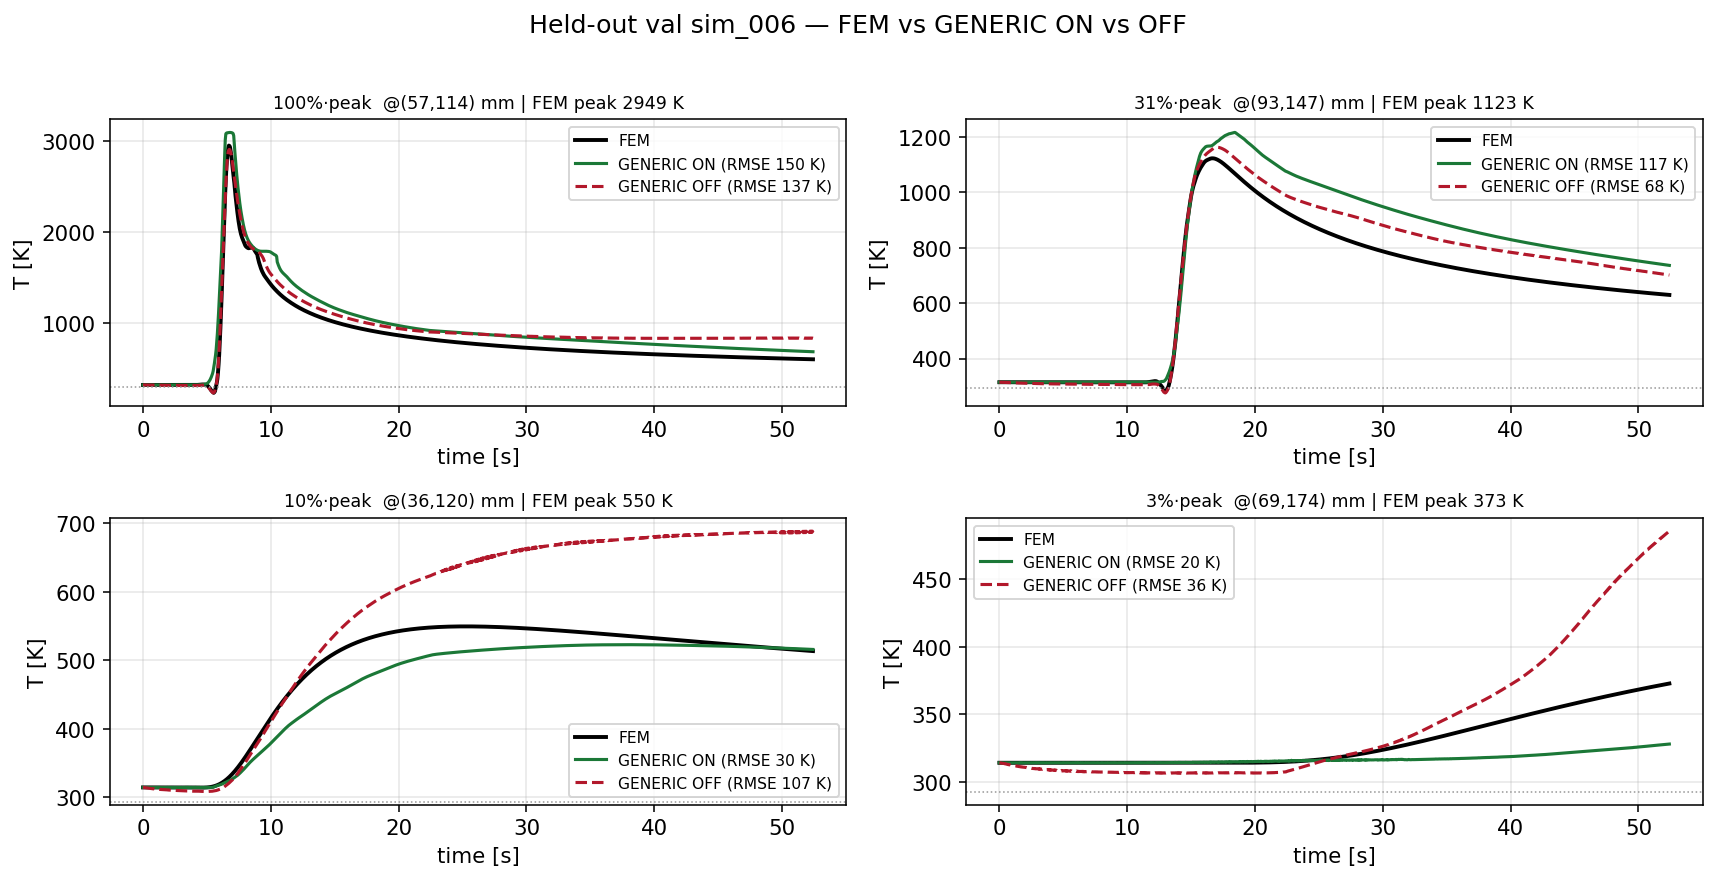
\includegraphics[width=0.92\linewidth]{compare_val_sim006_fem_on_off.png}
  \vfill
\end{frame}

%------------------------------------------------------------------ Spiral 1: setup + ParaView video
\begin{frame}{The Archimedean spiral: an out-of-distribution stress test}
  \restag{the spiral (OOD)}
  {\small \textbf{Spiral weld} (\SI{0.2}{m}, 3 turns, \SI{10}{mm/s}): a trajectory
  \textbf{never seen} in training, rolled out over \num{1526} steps.}
  \vfill
  \begin{center}
    \animategraphics[autoplay, loop, controls, poster=last, width=\linewidth]%
      {12}{spiral_frames/frame-}{0}{190}
  \end{center}
  \vfill
\end{frame}

%------------------------------------------------------------------ Spiral 2: histories + stability (combined)
\begin{frame}{Spiral results: thermal histories \& stability (ON vs.\ OFF)}
  \restag{the spiral (OOD)}
  \begin{columns}[c]
    \begin{column}{0.56\textwidth}
      \centering
      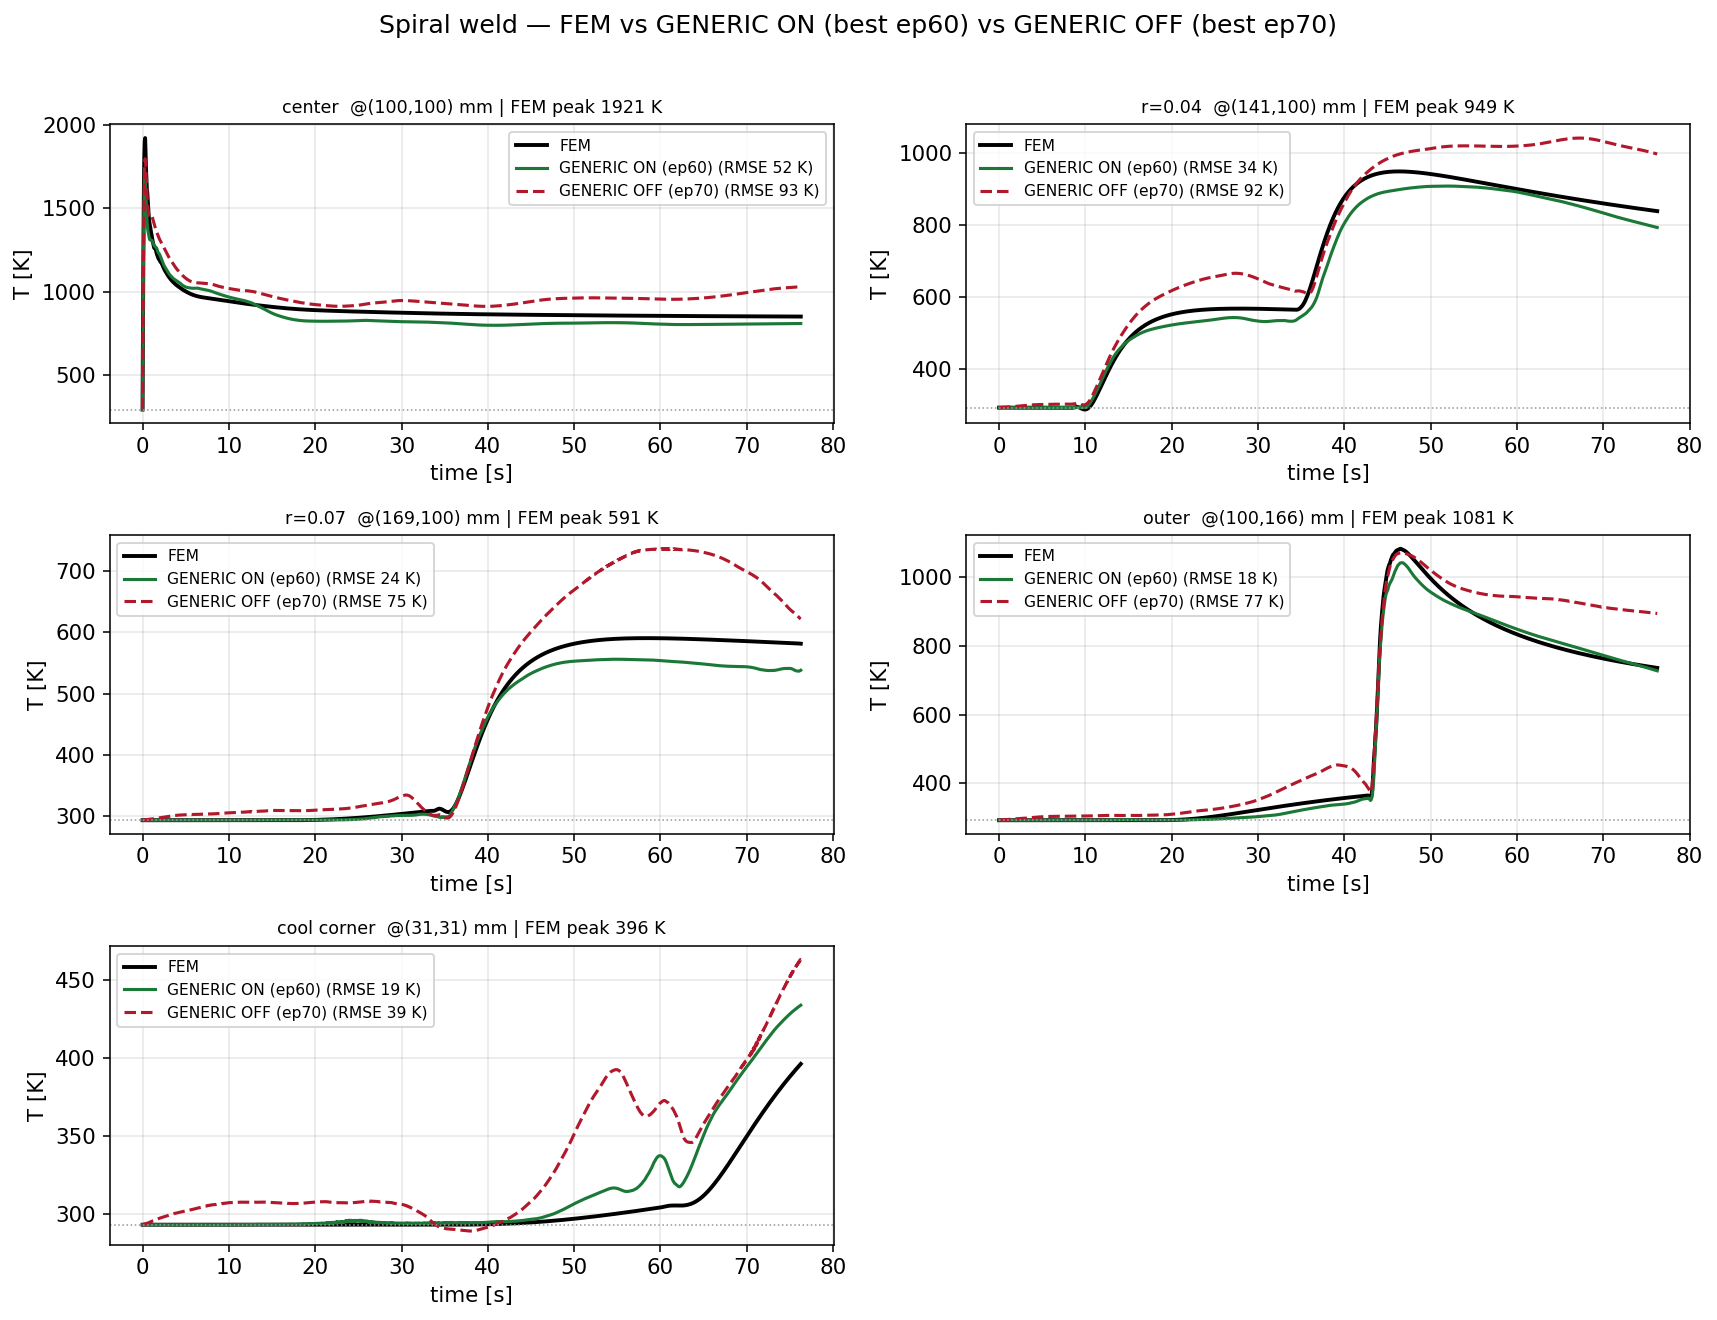
\includegraphics[height=0.84\textheight]{compare_spiral_fem_on_off.png}
    \end{column}
    \begin{column}{0.44\textwidth}
      \hfill
      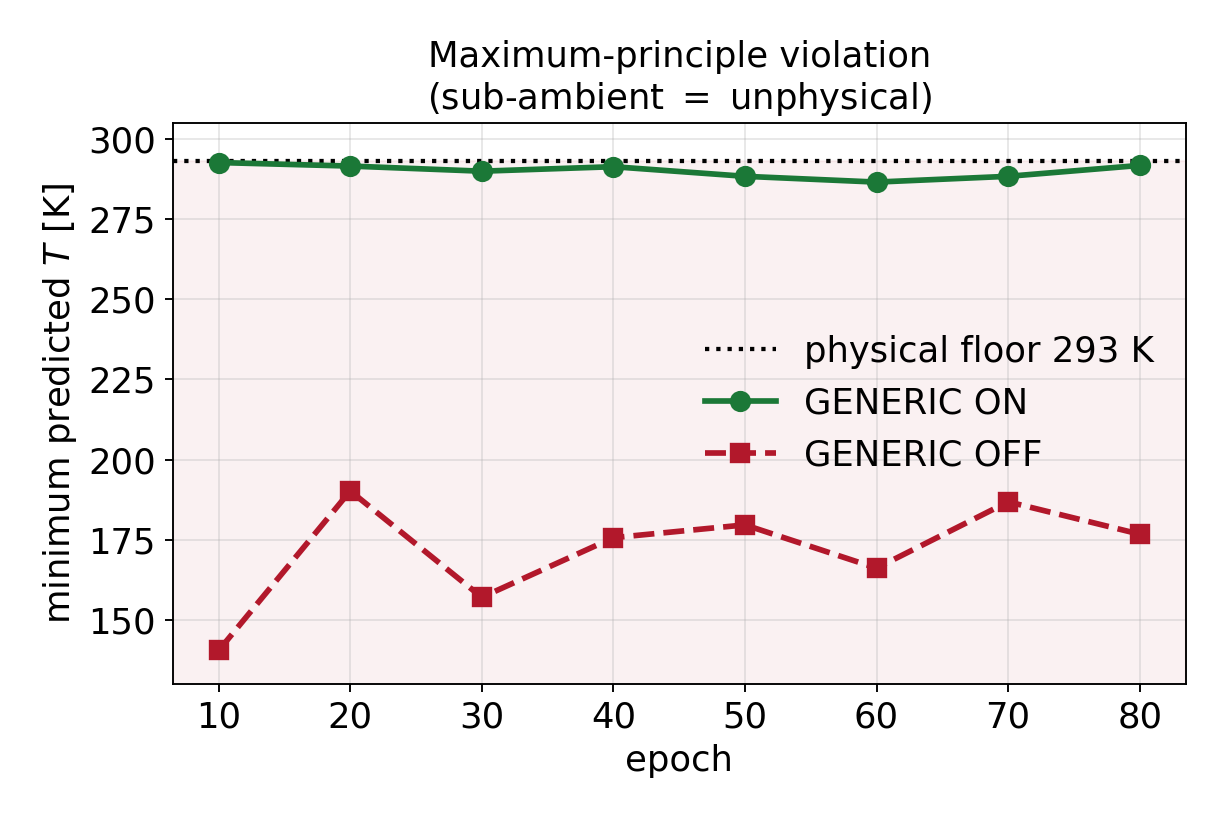
\includegraphics[width=0.82\linewidth]{ablation_minT.png}
    \end{column}
  \end{columns}
\end{frame}

%------------------------------------------------------------------ 13. conclusion
\begin{frame}{Conclusions}
  \textbf{Enthalpy-state GENERIC is a sound, thermodynamically-consistent
  formulation} for learned welding surrogates, and the structure both
  \textbf{guarantees the physics by construction} and \textbf{regularizes
  training}.
  \smallskip\pause

  \begin{itemize}[<+->]\itemsep2pt
    \item Energy (enthalpy) is the natural conserved state, so latent
      heat / phase change is handled \emph{exactly}; temperature via $T=h^{-1}$.
    \item 1st \& 2nd laws and the maximum principle hold \emph{every step, any
      mesh, any horizon}, not just at convergence.
    \item The structure \textbf{regularizes}: low-variance, \emph{selectable}
      checkpoints, stable \num{1526}-step rollouts, not accurate-but-fragile.
    \item \emph{Push-forward} $K{=}2$ aligns the objective with the long
      rollout; demonstrated OOD generalization to an unseen weld trajectory.
  \end{itemize}
  \smallskip\pause

  {\structure{\textbf{Work in progress.}}\ \small detailed training-set analysis;
  ablation of the push-forward steps $K$; generalization beyond trajectory
  (geometry / process / material, other regimes); 3D extension.}
  \smallskip\pause
  \begin{center}\structure{Thank you! Questions?}\end{center}
\end{frame}

\end{document}
